% Chapter Template

\chapter{Device fabrication and experimental methods} % Main chapter title

\label{Chapter5} 

\HRule
\vspace{0.5cm} \hspace{2cm}
\small
\hangindent=4cm
\\
        ``\emph{Scalability is the future}"
\\ \\
\hangindent=4cm
\begin{flushright}
--? \\
\end{flushright}

\vspace{0.5cm}

\noindent \HRule
\clearpage

\section{Device design} \label{sec:deviceDesign}

To propel the flip flop qubit from a theory proposal to reality, we are using nanofabrication techniques to build the qubit up from a blank silicon wafer for both dipole-dipole coupling and coupling to a superconducting resonator. Therefore we first need a design that fulfils all requirements of the flip flop qubit and complies with the fabrication tools available to us. 
From chapter \ref{Chapter2} we know that we need 
\begin{itemize}
\item Readout of the electron state
\item Control of the tunnel coupling 
\item Confinement of the electron at the interface
\item Electrical control of the donor with fast pulses
\end{itemize}

Additionally we would like an ESR antenna to be able to perform ESR and NMR to control the electron and nuclear spin states separately from any flip-flop control.  The following section describes how these requirements can be implemented for direct dipole coupling while section \ref{sec:designCPWR} discusses the circuit QED approach. 

\subsection{Flip-flop qubit} \label{sec:designFF}

\begin{figure}
	\centering
	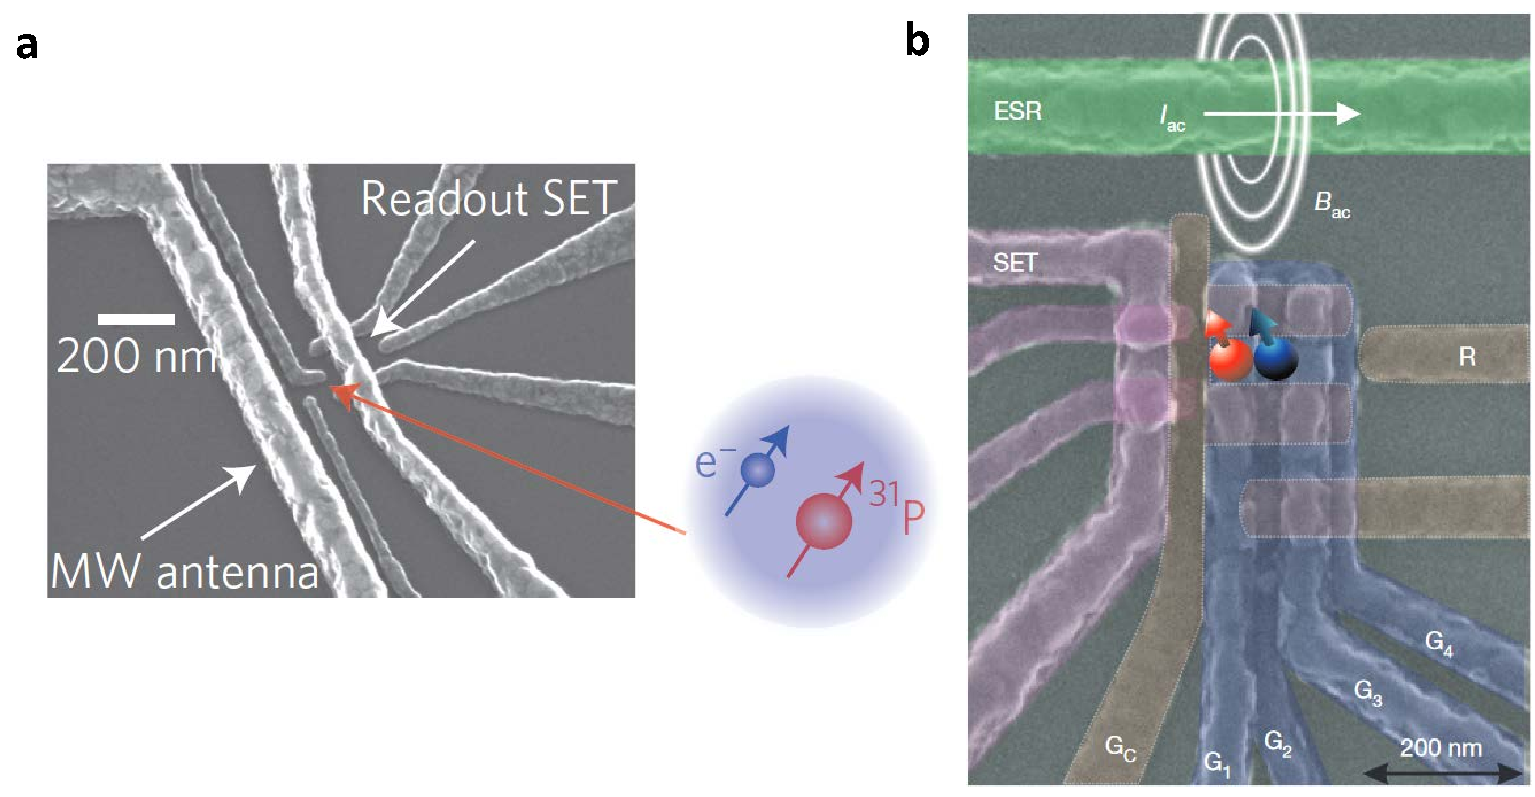
\includegraphics[width=0.7\textwidth]{polished/donorDot.pdf}
	\caption[Silicon donor and quantum dot qubit designs]{\textbf{Silicon donor and quantum dot qubit designs}. a }
	\label{fig:donorDotDevices}
\end{figure}

We base our flip-flop qubit structure on existing donor and quantum dot structures (figure \ref{fig:donorDotDevices}) that have made our research teams at UNSW very successful over the last decade \cite{Muhonen2014, Veldhorst2014}. We are working with donors in silicon but also separate the electron from the donor and confine it at the silicon interface - just like a quantum dot. Thus our flip-flop qubit will be a hybrid structure from the designs shown in figure \ref{fig:donorDotDevices} with generation one pictured in figure \ref{fig:designFF}a with a coloured layout on the left and an SEM image on the right. 

\begin{figure}
	\centering
	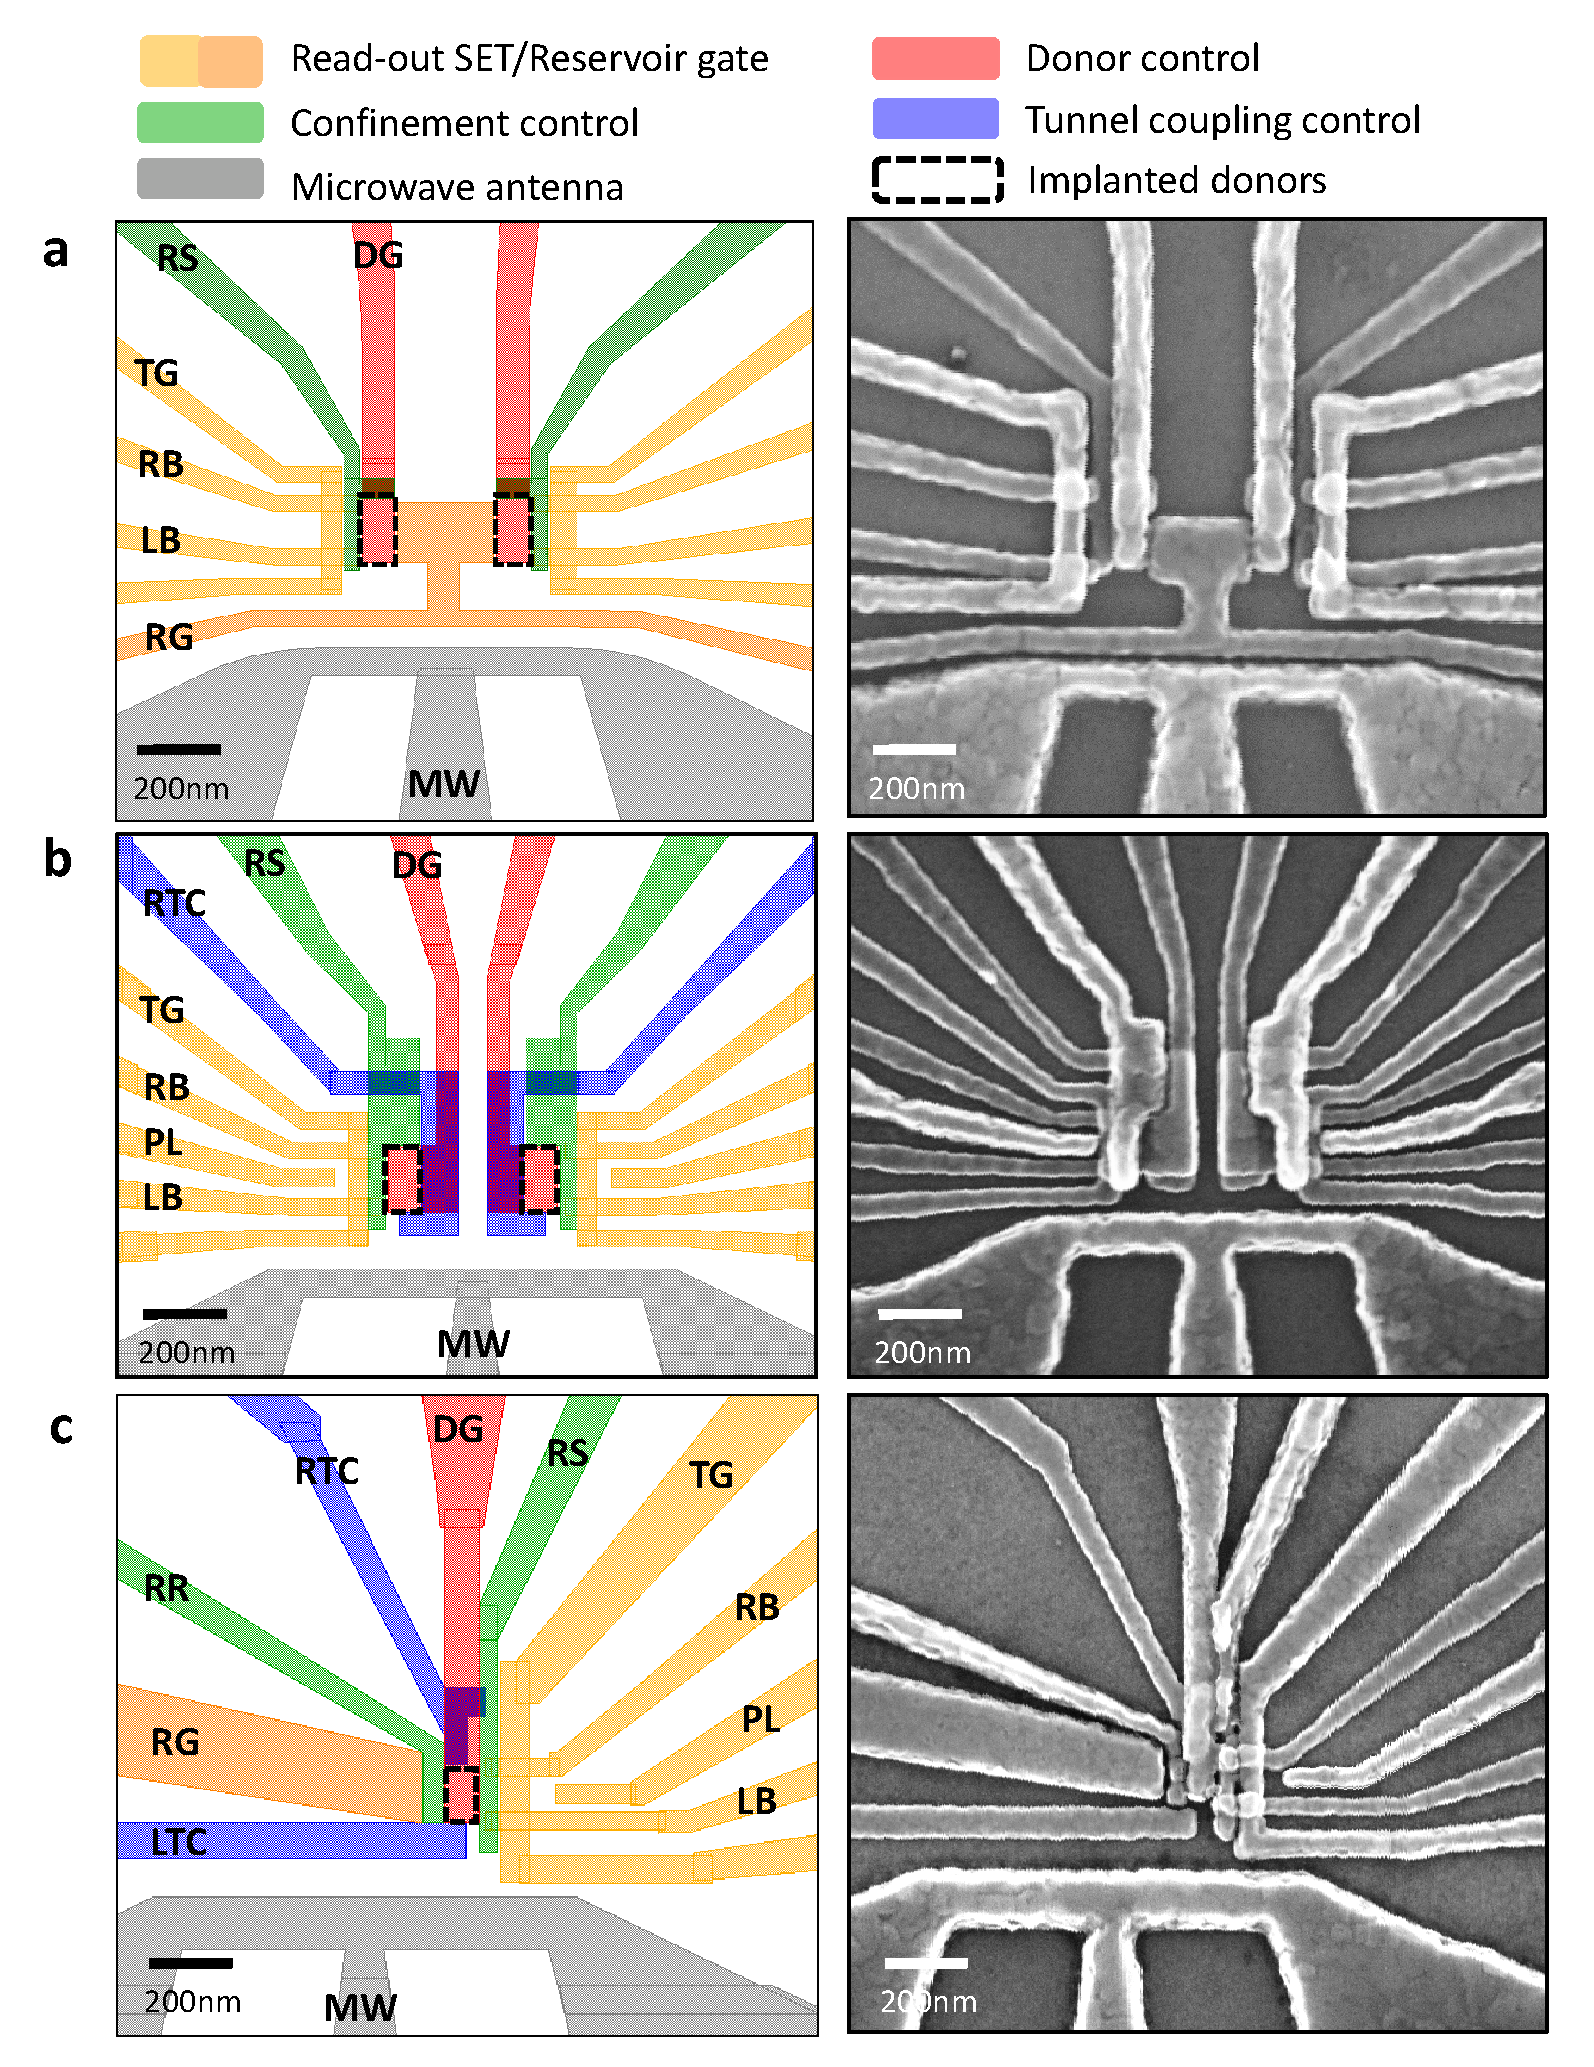
\includegraphics[width=\textwidth]{polished/FF_designs2.pdf}
	\caption[Flip flop design]{\textbf{a}. a }
	\label{fig:designFF}
\end{figure}

The key elements prominent in both donors and dots remain unchanged: We use a SET for electron readout (yellow), consisting out of a top gate and two barriers with contact to a positively doped region (see section \ref{sec:SET}), and a coplanar microwave antenna (grey) to supply the MW and RF magnetic fields. 
Now we add a rate gate between the donor and the SET (green), like in the QD devices, to control the tunnel rate of the electron to the SET and prevent escape of the interface state.  Additionally this gate can be used to tune the tunnel coupling. Lastly we add an impedance matched donor gate on top of the donor to control the donor state and send fast electric pulses. 
However, we encounter one problem: To tune the tunnel coupling significantly we need to pull the electron horizontally by up to $100\,$nm. Consequently we choose an implantation window size of $60\times120\,$nm as indicated in figure \ref{fig:designFF}. Together with the necessary rate gate, this can lead to far distances of the donor to the SET island though - too far for tunnelling. To account for this difficulty we add an additional reservoir. This brings two distinct advantages: Firstly, now any donor close to either the SET island or the reservoir can be read out with the traditional donor readout (see section \ref{sec:readout}). Secondly, if the dot cannot be readout from the donor, we can readout the interface (dot) state instead. As the dot energy is usually lower than the donor energy with $E_{d}=-45\,$mV, this requires a flexible Fermi level: Once we apply a bias voltage large enough to pull the dot state below the donor state, we need to adjust the Fermi level to only populate the dot state. This is illustrated in figure \ref{fig:ff_readout}. During this process the SET Fermi level stays constant to provide charge sensing. We mirror this one-qubit structure at a distance of $200\,$nm to achieve a two-qubit device.

In generation two (Fig. \ref{fig:designFF}b) we added a plunger gate (yellow) for better SET adjustment and an additional tunnel gate (blue) to have higher control over the tunnel coupling at cost of the reservoir gate. 

Generation three (Fig. \ref{fig:designFF}c) incorporates both high tunnel coupling control (blue gates) and high adjustability for electron readout in form of an additional reservoir, rate gates and a plunger gate. To achieve this highly controllable device however we had to sacrifice the second qubit. Thus this generations focus will be one-qubit performance.
A few general small design changes were made as well: The SET tunnel gate as well as the plunger gate have been moved further away from the SET top gate to reduce the effect of strain on the 2DEG below the SET as this can prevent turn-on. Furthermore, the microwave short has been increased in both width and hight to make it less susceptible to melting from sudden voltage fluctuations. 


\subsection{CPWR} \label{sec:designCPWR}
resonator designs over the years

\begin{figure}
	\centering
	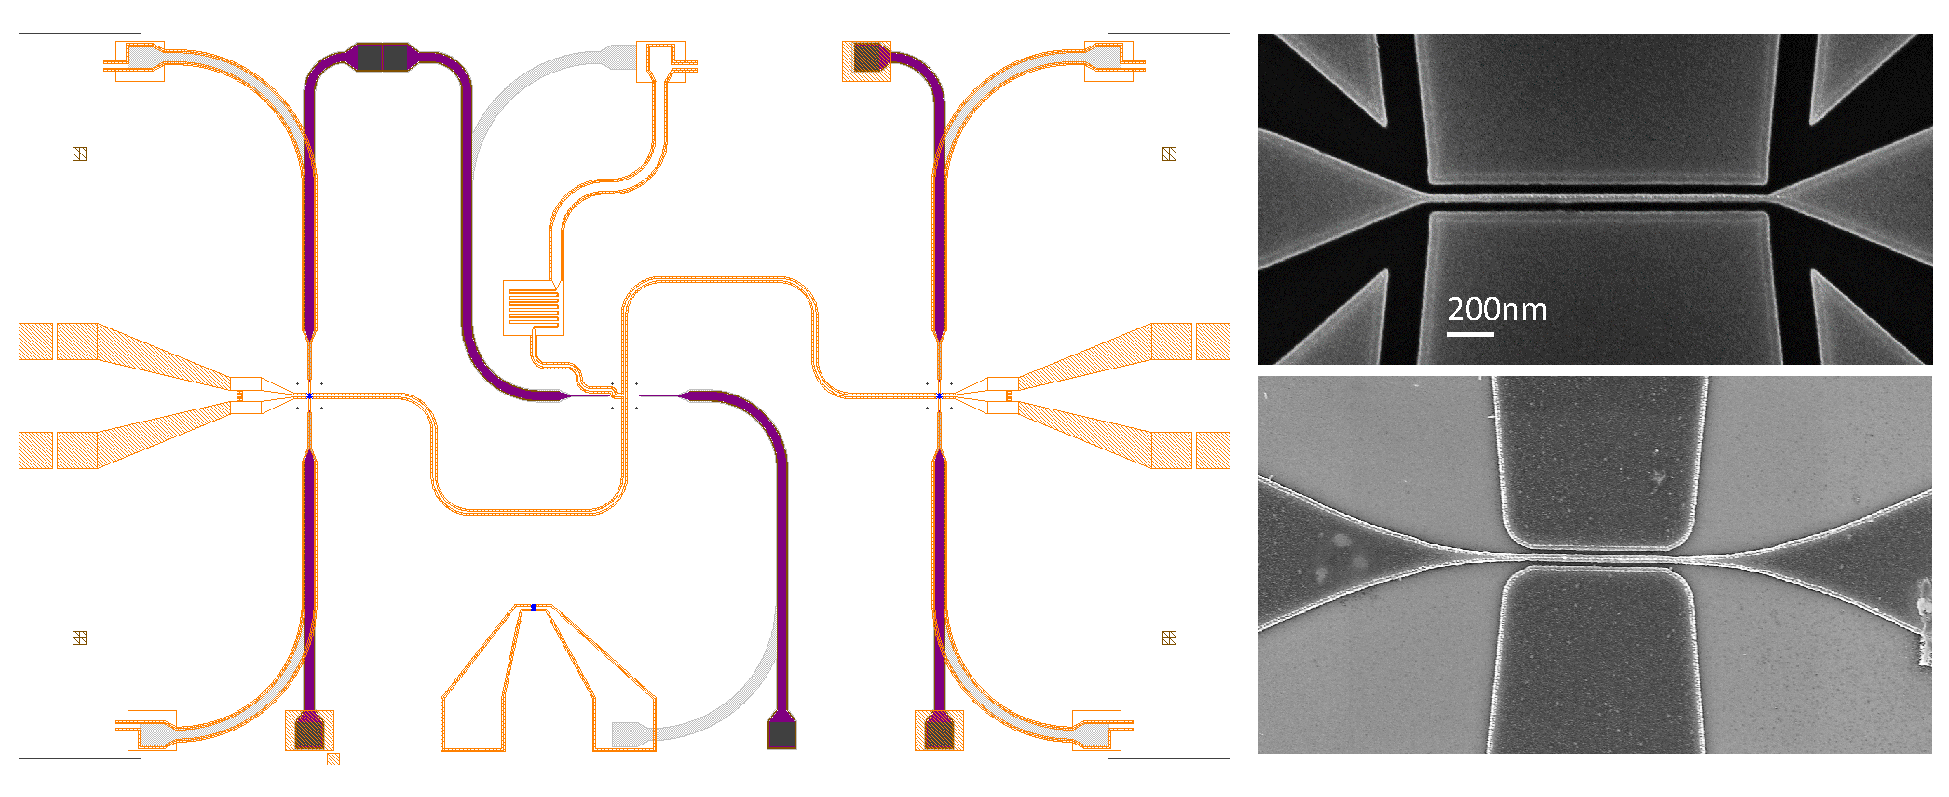
\includegraphics[width=\textwidth]{polished/CPWR_designs.pdf}
	\caption[Flip flop design]{\textbf{a}. a }
	\label{fig:designFF}
\end{figure}

second generation with AL


\section{Device fabrication} \label{sec:fabrication}

\subsection{Silicon wafer} \label{sec:fabWafer}

\begin{figure}
	\centering
	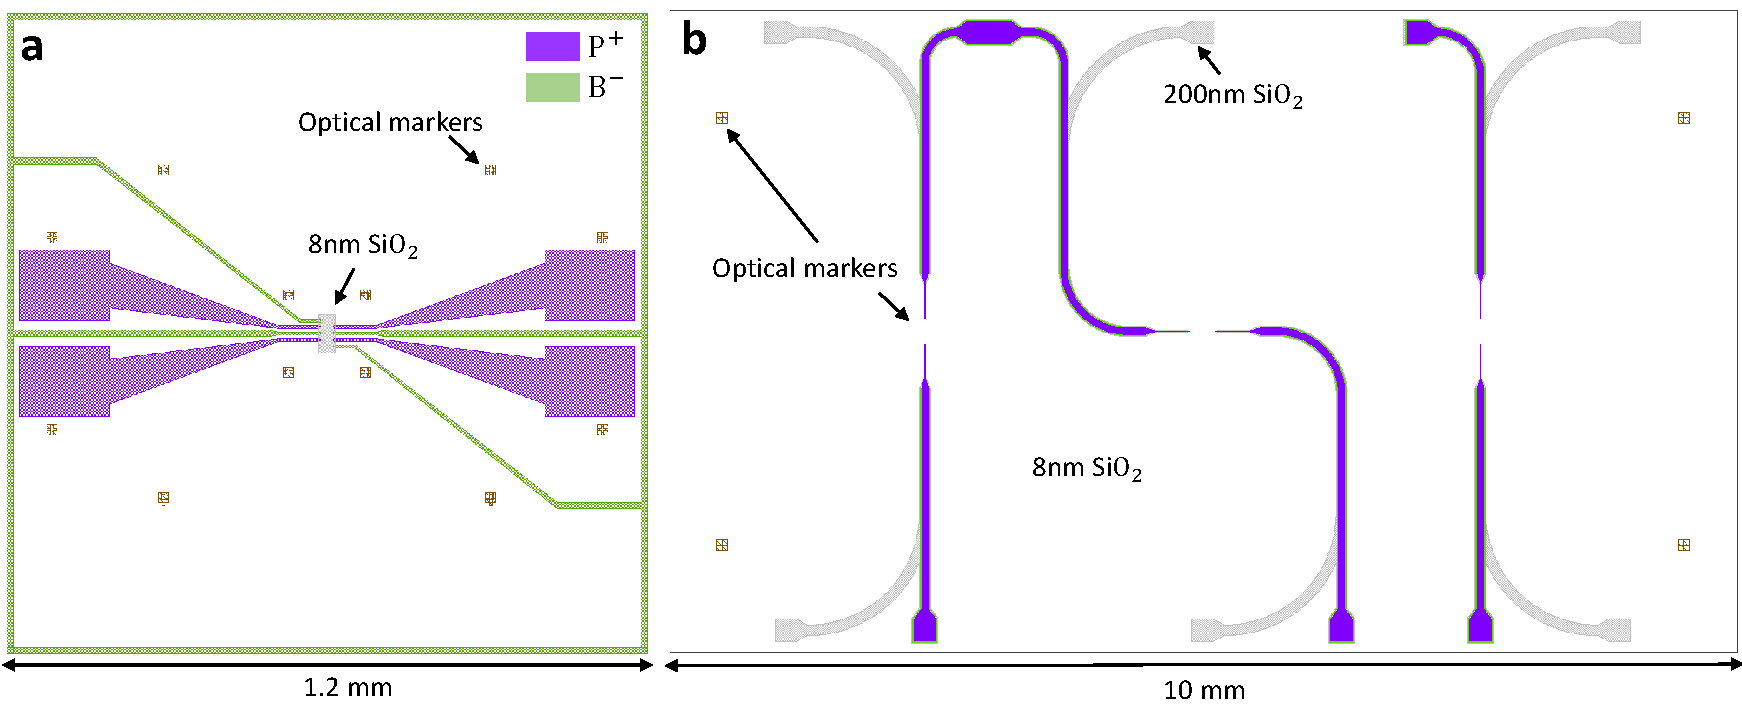
\includegraphics[width=\textwidth]{polished/stock.pdf}
	\caption[Silicon wafer layout]{\textbf{a}. a }
	\label{fig:wafer}
\end{figure}

All devices start off as a bare silicon wafer. For testing natural silicon wafers with low residual p-type background doping ($\sim 10^{12}\,\rm{cm}^{-3}$) are used, while highly precise qubit experiments are performed on wafers with an $800\,$nm epitaxial layer of isotopically purified $^{28}$Si on top of $500\,\mu$m thick high purity natural silicon, provided by K. Itoh. The $^{28}$Si has a residual concentration of $730\,$ppm of $^{29}$Si and $30\,$ppm $^{30}$Si.
The first step after acquiring a new wafer is a thorough clean. Then optical alignment marks are etched into the silicon. Next the wafers are doped firstly with Boron ($B^-$) to create positively charged guard rings. These guards prevent leakage at the Si-SiO$_2$ interface when positive charges trapped in the field oxide induce an unintentional two-dimensional electron gas (2DEG). Then phosphorus ($P^+$) is diffused to create $n+$ regions to form the source and drain contacts. Afterwards $200\,$nm of field oxide are grown in a wet thermal oxidation furnace. Following the field oxide is reduced in the active qubit region to be replaced by a $8\,$nm ($2\,$nm for CPWR style devices) of high quality gate oxide, grown in an ultra-dry furnace. Lastly micrometer sized markers formed out of Platinum on top of Titanium (TiPt markers) are patterned for course alignment with electron beam lithography (EBL). Figure \ref{fig:wafer}a shows an image of a standard qubit wafer after this initial processing. 

The processing of wafers designated for coupling to superconducting resonators is done in the same way. The only noticeable difference is that most of the wafer is the active region and thus only where the top gates will be running thick oxide is grown. This wafer design is shown in figure \ref{fig:wafer}b. 


\subsection{Nano-fabrication process - aluminium devices}

Once the silicon wafers have been prepared, they are diced into smaller chips for different projects. All silicon donor aluminium style devices use inherently a very similar fabrication process. In the following the process specific to the flip-flop qubit used in this thesis is presented. 
\paragraph*{Cleaning}
To remove any residue of resist or other contaminants the chips are cleaned by soaking them first in acetone and subsequently in Isopropyl alcohol (IPA) for each 10 min while applying ultrasound. The cleaning process is finished with 10 min of oxygen plasma ashing. 

\begin{figure}
	\centering
	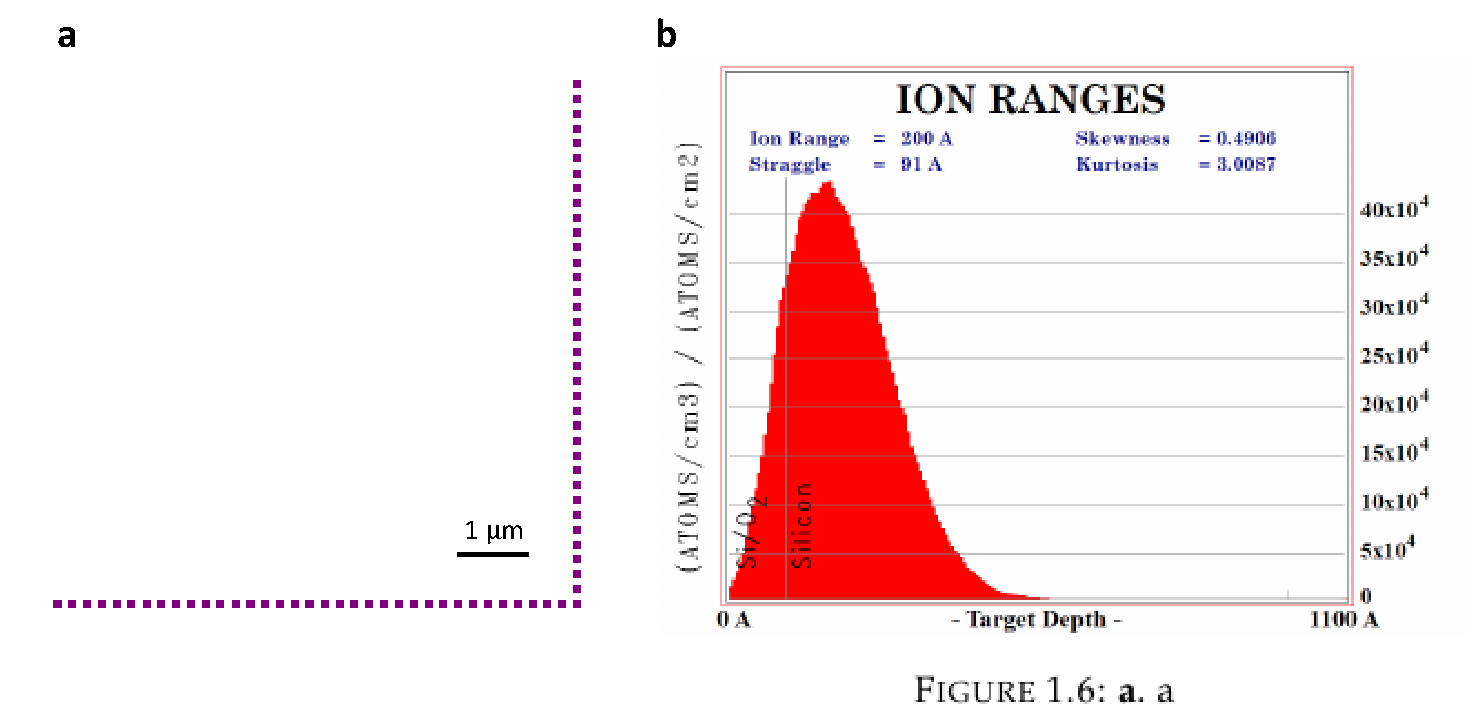
\includegraphics[width=\textwidth]{polished/implantion_TiPtmarks.pdf}
	\caption[TiPt]{\textbf{a}. a }
	\label{fig:TiPtmarks_impl}
\end{figure}

\paragraph*{TiPt markers}
The first processing step is the addition of the nanometric markers in each pixel which enable alignment of different layers during EBL. These markers need to withstand temperatures of $1000\,\degree$C during subsequent processing steps. Therefore we use Platinum which not only has a very high melting point of $1763\,\degree$C but also has a high atomic number resulting in good contrast on the electron beam microscope. For adhesion to the silicon oxide surface we add a thin layer of Titanium with a melting point of $1668\,\degree$C. Regardless of these high melting points, large TiPt structures melt and deform. Consequently we use marker shapes consisting out of many small $100\times100\,$nm squares as shown in figure \ref{fig:TiPtmarks_impl}a which survive our high temperature process. We create these markers using EBL. There we first bake our chip at $180\,\degree$C for 10 min and then spin polymethyl methacrylate (PMMA) A4 resist with $4000\,$rpm for 40s with 10s of $8000\,$rpm finish. This gives a resist thickness of $200\,$nm. The resist is then baked for 90s at $180\,\degree$C. Droplets of colloidal gold solution can be placed on the corners of the chip as focus markers. The pattern is written with a RAITH150-Two EBL system with an acceleration voltage of $30\,$keV and a dose varying around $500\mu C/cm^2$, depending on aperture, feature size and geometry. After exposure, the resist is developed for 40s in a 1:3 solution of methyl-sobutyl-ketone (MIBK) and IPA and for 20s in IPA with a 5s ultrasound finish. 
Subsequently 15nm of Titanium and 65nm of Platinum are evaporated by electron beam physical vapour deposition (EBPVD). Then the chip is placed in N-methyl-2-pyrollidone (NMP) at $80\,\degree$C for 5min to perform lift off. 

\paragraph*{Donor implantation}
The next step is the implantation of our phosphorus donors. Therefore a PMMA mask of dimensions  $120\times60\,$nm is patterned with EBL in each pixel (implantation window). We require a donor depth of around 10-15nm below the silicon oxide. As the tunnel coupling between the donor and dot can be reduced but not increased we aim for 10nm. An acceleration voltage of 12keV of $P^+$ ions complies with this requirement as the simulated ion depth distribution in figure \ref{fig:TiPtmarks_impl}b shows. We'd like 8-10 donors in our implantation window which corresponds to a fluence of $2\cdot 10^{11}/cm^2$ and an average donor distance of 25nm. The implantation is performed by Jeff McCallum. After the implantation is completed the resist is removed and the chip undergoes rapid thermal annealing (RTA) for 5s at $1000\,\degree$C. This activates the donors and repairs the damage caused in the silicon lattice by the ion implantation \cite{McCamey2005}. Finally Aluminium Ohmic contacts to the diffused $n+$ regions are formed and activated with a forming gas anneal (FGA) (N$_2\ 95\%$, H$_2\ 5\%$) at $400\degree$C for 15min in the clean anneal furnace and the chip is diced into 4x4 pixel pieces for individual processing. 

\paragraph*{Multi-layer Aluminum nanostructures}

\begin{figure}
	\centering
	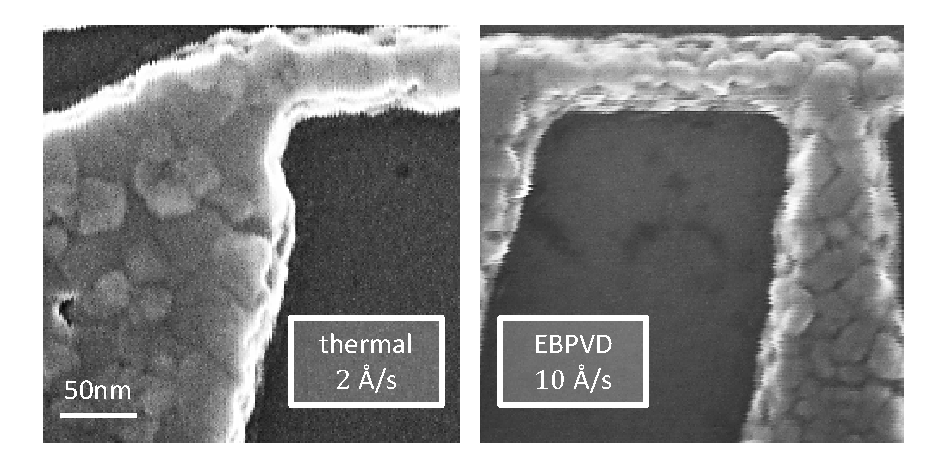
\includegraphics[width=0.7\textwidth]{polished/grainsize.pdf}
	\caption[grain size]{\textbf{a}. a }
	\label{fig:grainsize}
\end{figure}

On each 4x4 pixel piece three layers of aluminium gates on top and around the implantation window are now added. For each layer the piece undergoes the following steps. 
First the piece is cleaned, then PMMA resist is spun and exposed during EBL as described above for the TiPt markers. After development aluminium is evaporated either in a thermal or an EBPVD evaporator. Tests have shown that the evaporation rate and its stability directly influences the aluminium grain size. Thermal evaporation can be unstable due to a fluctuating current and is restricted to rates below $3\,$\AA/s. Thus it regularly leads to a larger grains than EBPVD where evaporation rates of $10\,$\AA/s can be achieved - see figure \ref{fig:grainsize}. With EBPVD we evaporate 25nm, 45nm and 80nm subsequently for the different layers and lift off in hot NMP for 1.5-3h. During the following oxygen plasma ash and baking, the outer $2-3\,$nm of each aluminium layer are oxidized to form an electrically insulating layer. Figure \ref{fig:ff_layers} shows the layer schematic and each layer individually during a dose test. 

\begin{figure}
	\centering
	\includegraphics[width=\textwidth]{polished/FF_layers.pdf}
	\caption[SEM FF]{\textbf{a}. a }
	\label{fig:ff_layers}
\end{figure}

\paragraph*{Finish}
After the last layer has been completed, the piece is cleaned one more time and FGA is performed to passivate any charge traps at the Si-SiO$_2$ interface\cite{Brower1988}.

\subsection{Nano-fabrication process - superconducting devices}

As our research group had not fabricated any form of superconducting devices before, we started building up a new process which is still undergoing development. This section describes the fabrication performed for the measurements presented in this thesis and gives an outlook for new, more sophisticated resonator devices. 

\paragraph*{Cleaning} 
First the wafer is cleaned in the same way as for the aluminium devices. However, once the niobium layer has been deposited, oxygen ashing oxidises the niobium to a degree that compromises the quality of the superconducting film, thus will not be performed.

\paragraph*{Donor implantation}
The next step is the implantation of our phosphorus donors. Therefore a photo mask of dimensions  $44\times24\,\mu$m is patterned with photo-lithography in each pixel (implantation window). We implant $P^+$ ions with an acceleration voltage of 11keV and a fluence of $1\cdot 10^{11}/cm^2$ which corresponds to an average donor distance of 38nm. The implantation is performed by Jeff McCallum. After the implantation is completed the resist is removed and the wafer undergoes RTA. Finally Aluminium Ohmic contacts to the diffused $n+$ regions are formed and activated with a FGA.

\paragraph*{Sputtering}
First we apply a thin layer of Al$_2$O$_3$ to serve as an etch stopper. With atomic layer deposition (ALD) we run 30 cycles at $250\,\degree$C which gives 3 nm. 
Then the wafer is sent to CSIRO at Lindfield where the 50nm of niobium are sputtered. However, the film thickness fluctuates between $30-40\,$nm which is determined with a stylus profilometre. Using a 4-point measurement we find these films to have a resistance of $15\,\Omega$ at room temperature. 

\paragraph*{Resonator structures}
To pattern our resonator structures we spin PMMA resist and expose it with EBL. In contrast to the aluminium style devices, we write what will be removed. Moreover, the resonators are larger than one write field. To create a smooth coplanar waveguide we employ the fixed beam moving stage (FBMS) technique that moves the stage below the beam for the entirety of the device, thus apprehending stitching issues. After patterning we develop the sample. Then we perform hollow cathode reactive ion etching (HC RIE) with a gas mixture of 20sccm CF$_4$ and 10sccm Ar at a pressure of 5Pa with 50W power to remove the Nb not protected by our PMMA mask. This process needs to be carefully calibrated so that after the etch duration the Nb is fully removed but the PMMA mask is still protecting the remaining Nb surface. For this purpose we always add test samples to the process. After etching the sample is cleaned and ready for packaging. 

\paragraph*{Outlook}
Vivi stuff


\section{Device packaging} \label{sec:packaging}

\begin{figure}
	\centering
	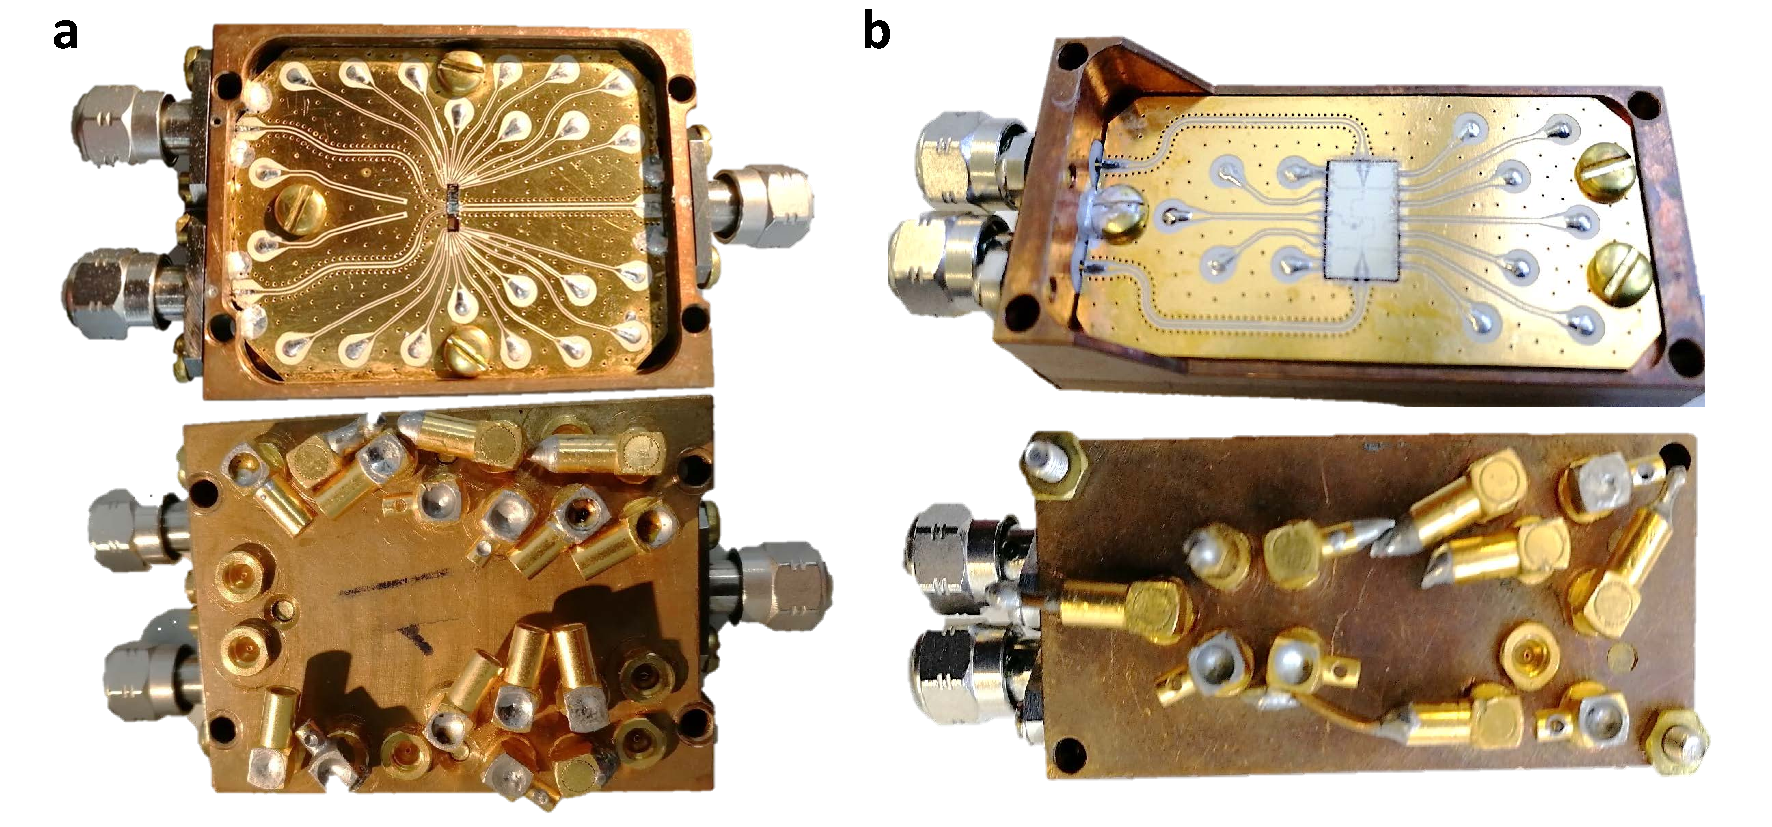
\includegraphics[width=\textwidth]{polished/PCB.pdf}
	\caption[PCB]{\textbf{a}. a }
	\label{fig:pcb}
\end{figure}

To connect our samples to electronics we use a printed circuit board (PCB) inside a copper enclosure as shown in figure \ref{fig:pcb}. These PCBs have been carefully designed with impedance matched lines for all high frequency ports and spare ports to accommodate for design changes. The dipole PCB (Fig. \ref{fig:pcb}a) holds two pixels which makes chip handling slightly easier as the pixel size is only $1.4\times1.4\,$mm. It features two high frequency SMA
and one SK line and 22 MMCX lines. The CPWR PCB (Fig. \ref{fig:pcb}b) holds one pixel and has two SMA and 12 MMCX lines. 

The device is mounted in the PCB opening with PMMA and subsequently connected to the PCB lines with an aluminium wedge wire bonder. Fast frequency lines are bonded as matched as possible by using many short bonds. The CWPR requires many additional bonds (from PCB ground to sample ground and across the different ground sections on the sample) to properly secure the ground plane is equal over the entire chip. During the bonding process all lines remain grounded to avoid electrostatic discharge (ESD) damage. 

\section{Experimental setup}

The enclosures with our qubits are mounted on a cold finger attached to the mixing chamber plate of a BlueFors cryogen-free dilution refridgerator. The fridge is outfitted with a superconducting magnet. The qubit sits in the center of the magnet and thus experiences a homogeneous magnetic field of up to 5 T.  The typical mixing chamber temperature is $12\,$mK. 

In this thesis three different types of qubits are discussed: the standard electron and nuclear qubit (see chapter \ref{Chapter1} and \ref{Chapter7}) and the flip-flop qubit with is implemented with direct dipole-dipole coupling and resonator coupling (see chapter \ref{Chapter2, Chapter3, Chapter4, Chapter6}). These different qubits have different demands on the measurement setup which will be explained in the following sections. 

\subsection{Cables and filtering}

\paragraph{Electron and nuclear qubit}

The qubit has three distinct types of connections to the room temperature world outside of the dilution refridgerator: DC, AC and high frequency ($>80\,$MHz) lines. Each type of connections aims to allow a sufficient amount of power down to the qubit while simultaneously minimizing any thermal conductance from the outside. Figure \ref{fig:queenie_filtering} shows the schematic of the fridge filtering used to achieve this aim. 

\begin{figure}
	\centering
	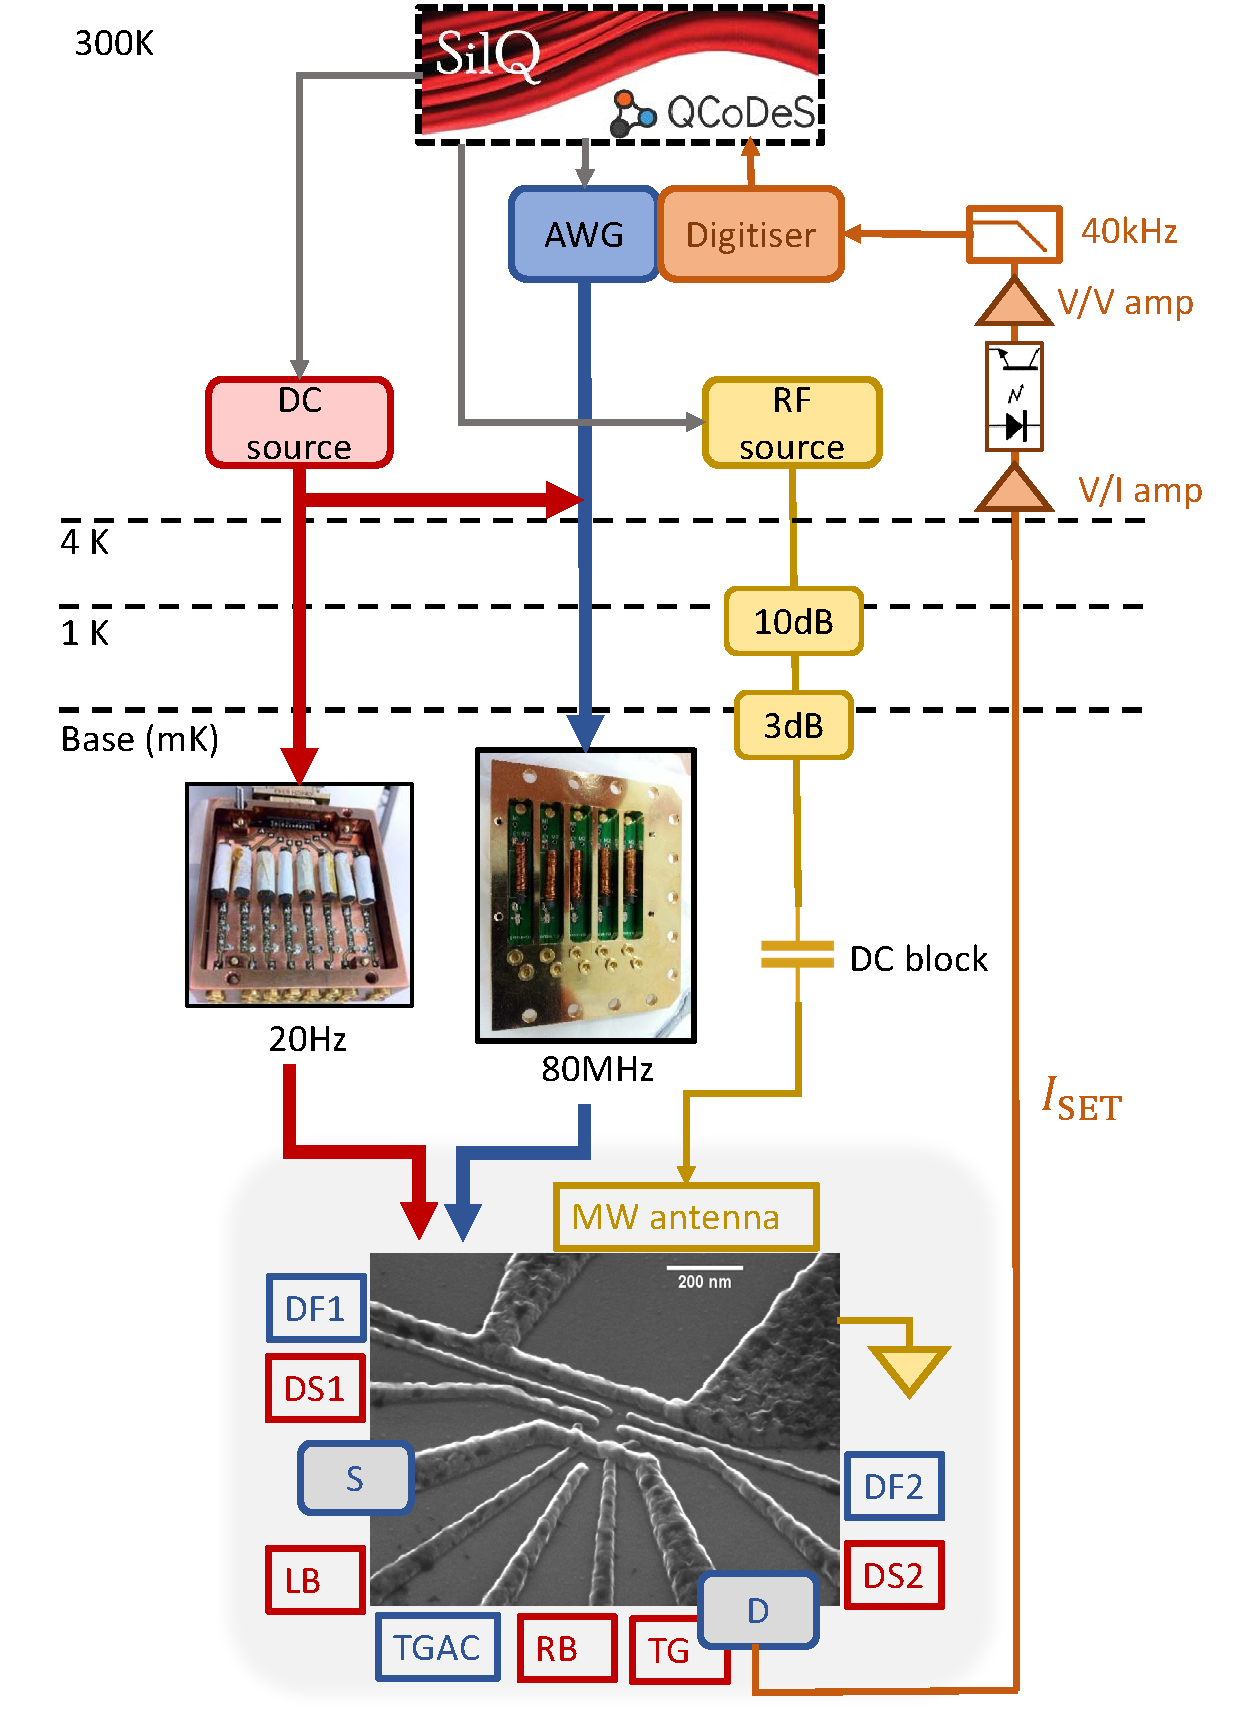
\includegraphics[width=0.8\textwidth]{polished/wiring_queenie.pdf}
	\caption[queeni filtering]{\textbf{a}. a }
	\label{fig:queenie_filtering}
\end{figure}

The DC lines consist out of the left (LB and right (RB) SET barrier, the SET top gate (TG), and two donor gates (DS1, DS2). These lines are connected to a handmade filter box that acts as a low pass filter and attenuates any signal above 20 Hz. It consists out of two passive
first-order RC filters in series with thin-film nichrome resistors of $20\,k\Omega$ and $470\,$nF and $1\,$pF ceramic capacitors, resulting in cut-off frequencies of $20\,$Hz and $8\,$MHz respectively. 

%johnson noise

\begin{figure}
	\centering
	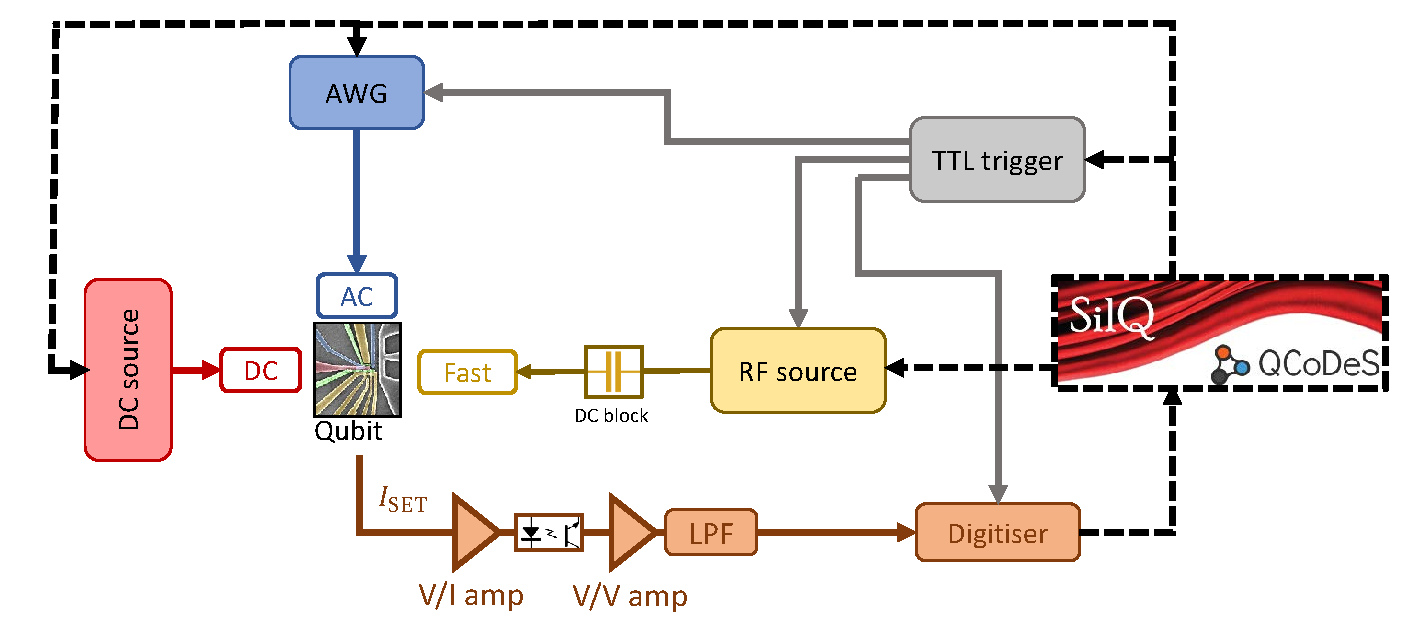
\includegraphics[width=\textwidth]{polished/RTsetup.pdf}
	\caption[queeni filtering]{\textbf{a}. a }
	\label{fig:queenie_rtsetup}
\end{figure}

qcodes / silq

\paragraph{Flip flop qubit}

While this qubit setup is very similar to the standard electron qubit setup, there are quite a few distinct differences which have been specifically designed for this project. 

\begin{figure}
	\centering
	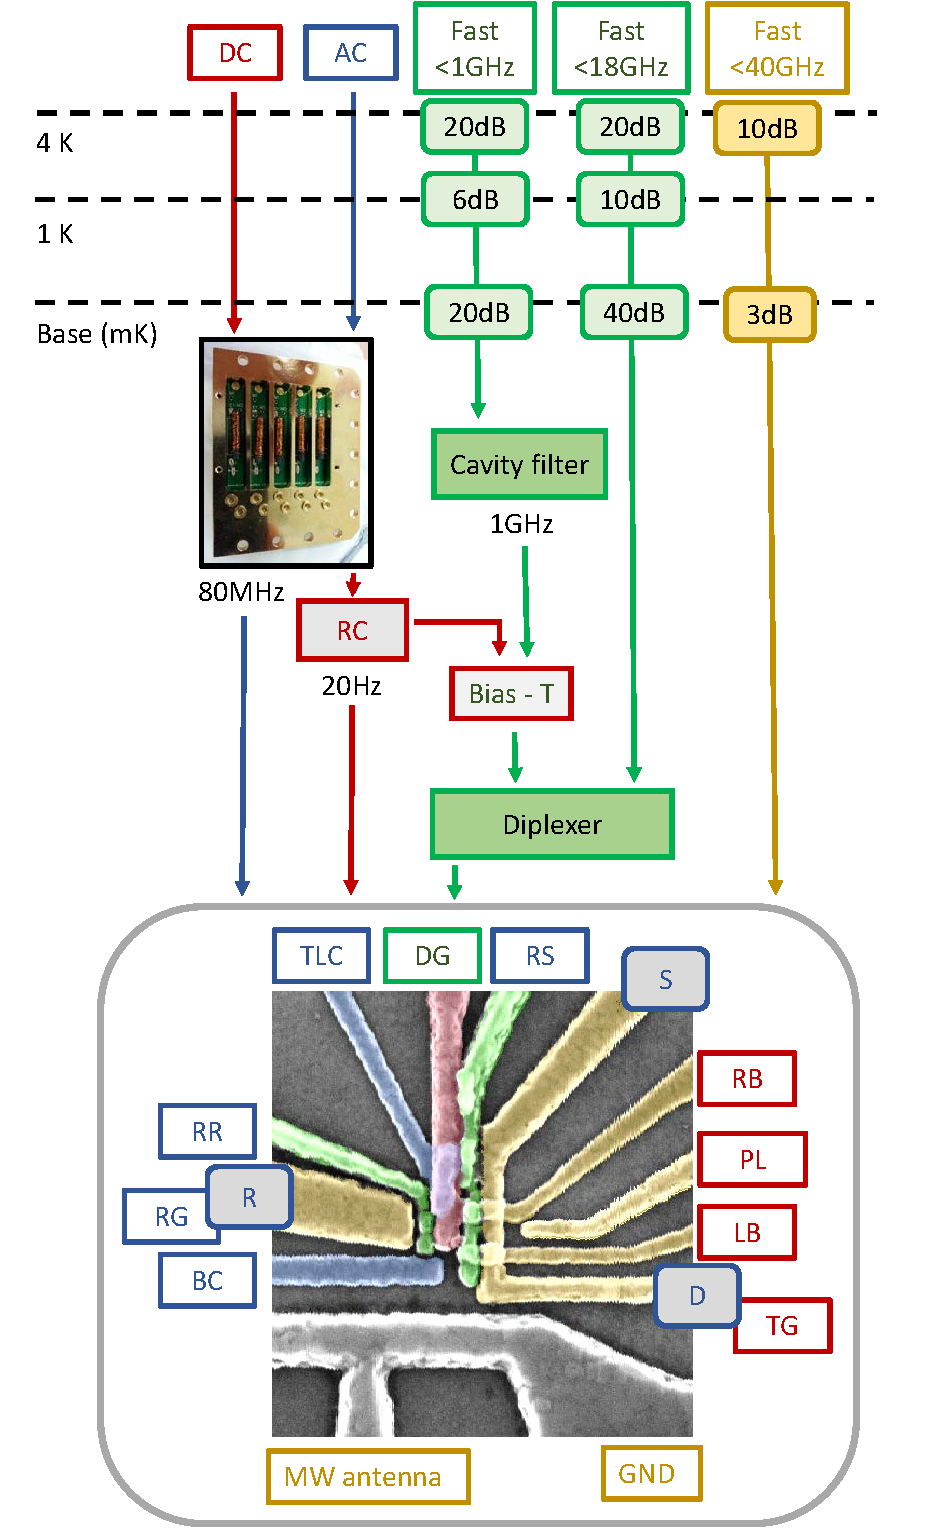
\includegraphics[width=0.8\textwidth]{polished/wiring_ff.pdf}
	\caption[ff filtering]{\textbf{a}. a }
	\label{fig:sem_ff_v1}
\end{figure}

\begin{figure}
	\centering
	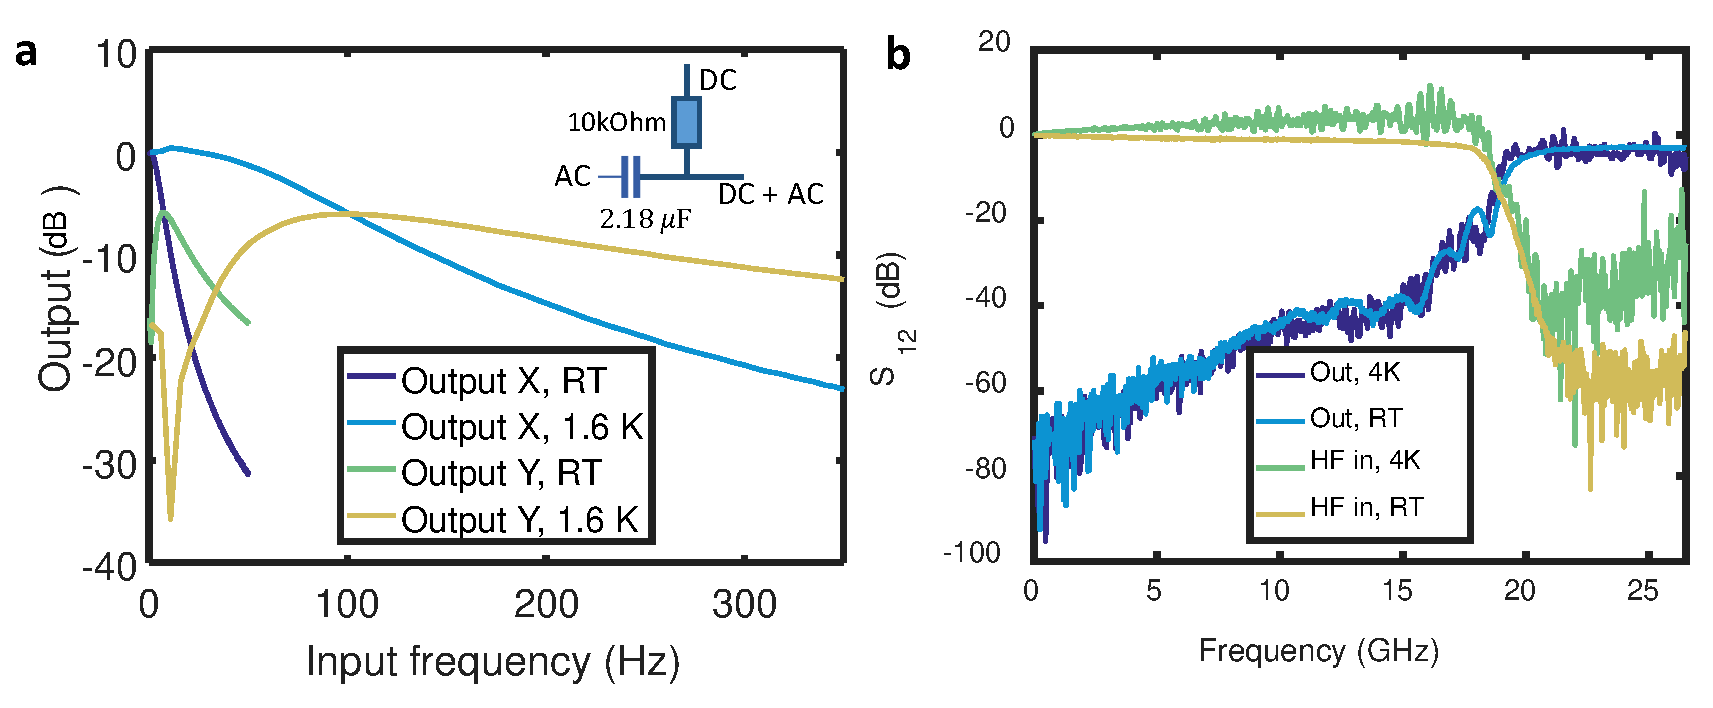
\includegraphics[width=\textwidth]{polished/ff_filtering.pdf}
	\caption[ff filtering]{\textbf{a}. a }
	\label{fig:sem_ff_v1}
\end{figure}

BT measurements
diplexer measurement

any other fridge measurements?

\paragraph{CPWR}
resonator readout

circulator stuff idk



